\chapter{Compiler}
Programmiersprachen dienen als Verständigungsmittel zwischen Programmierern und Rechenanlagen. Diese Sprachen haben sich in der Vergangenheit dabei immer mehr an die  Terminologie eines bestimmtes Anwendungsgebietes angenähert. Durch diese Entwicklung eigneten sich Programmiersprachen direkt für die Dokumentation von entwickelten Algorithmen und Anwendungen, entfernten sich jedoch weiter von den Gegebenheiten des realen Rechners.\footcite[Vgl.][S. 15]{Schneider1975}
\begin{figure}[h]
 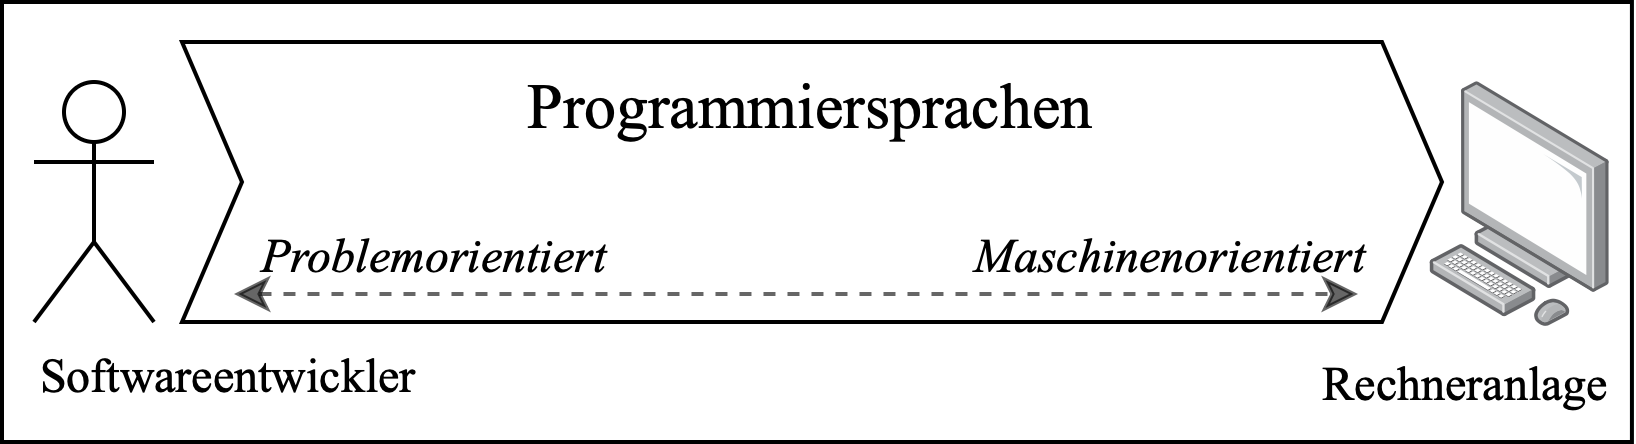
\includegraphics[width=\textwidth,height=\textheight,keepaspectratio]{Images/LanguageIntermediary.png}
 \caption{Programmiersprachen als Schnittstelle}
 \label{fig:Programmiersprachen als Schnittstelle}
\end{figure}
Für die Ausführung einer in einer problemorientierten Programmiersprache geschriebenen Anwendung ist es notwendig, die Sprache in eine maschinenorientierte Form zu überführen. \footcite[Vgl.][S. 15]{Schneider1975} Bereits im Jahre 1952 stelle Rutishauser fest,  dass Computer in der Lage sind diesen Übersetzungsvorgang selbst durchzuführen.\footcite[Vgl.][S. 312]{Rutishauser1952} 
Durch die Möglichkeit zur automatischen Übersetzung von problemorientierten Programmiersprachen konnten Hochsprachen entwickelt werden, die menschenfreundliche Sprachelemente anstatt Maschineninstruktionen verwenden. \footcite[Vgl.][S. 47]{Wagenknecht2014}
\section{ Grundbegriffe}
Diese historische Einführung zeigt,  dass Software zur automatisierten Übersetzung schon seit der Mitte des letzten Jahrhunderts thematisiert wurde, so hat sich in der Wissenschaft eine einheitliche Definition ergeben.  \citeauthor{Ullmann2008} beschreibt die sogenannten Compiler im Jahre \citeyear{Ullmann2008} wie folgt:\footcite[Vgl.][S. 1]{Ullmann2008} 
\begin{Def}[Compiler]
Ein Compiler ist ein Programm, welches ein anderes Programm aus einer Quellsprache in ein gleichwertiges Programm einer Zielsprache übersetzen kann.
\end{Def} 
\vspace{-1em}

Aus dieser Definition lässt sich ein für diese Arbeit relevanter Fakt ableiten: Compiler sind nicht ausschließlich Übersetzer zwischen zwischen problemorientierten,- und maschinenorientierten Programmiersprachen.  Sie sind ausschließlich für die Übersetzung von einer Quellsprache in eine Zielsprache verantwortlich.  Auch wenn der Begriff Programm für jedermann geläufig ist,  kann es dennoch passieren,  das von verschiedenen Repräsentationen eines Programmes gesprochen wird.  So können alle drei der folgenden Begriffe als Programm bezeichnet werden: Der Quelltext, dass ausführbare Programm kann er dennoch unterschiedliche Repräsentationen eines Programmes meinen.  Für das weitere Verständnis dieser Arbeit ist,  mit dem Begriff Programm die ausführbare Anwendung auf den Smartphones des Anwenders gemeint.  

Neben der Übersetzung von problem zu maschinenorientierter Sprache gibt es ebenfalls Compiler, die andere Ziele verfolgen. Dazu gehört zum Beispiel die sogenannten Binärübersetzer,  die den Binärcode eines Programmes für andere Rechner übersetzen, sodass er auf diesen ausgeführt werden kann.  \footcite[Vgl.][S. 27]{Ullmann2008} Ein Source-to-Source(S2S) Compiler,  häufig auch als "Transpiler" bezeichnet,  ist ebenfalls eine besondere Ausprägung eines Compilers die sich wie folgt definieren lässt.  \footcite[Vgl.][S. 1629]{IJCSIT2015}
\begin{Def}[Source-to-Source Compiler]
Ein Source-to-Source-Compiler ist ein Compiler, bei dem sowohl die Quellsprache als auch die Zielsprache eine Hochsprache ist.
\end{Def}
\vspace{-1em}

Der Begriff Hochsprache ist dabei ein Synonym für die bereits eingeführten problemnahen Sprachen wie zum Beispiel C++,  Java,  C\# oder Dart und damit für den Menschen in einer lesbaren und änderbaren Form geschrieben sind. \footcite[Vgl.][S. 9]{Eisenecker2008} 

\section{Compiler Struktur}
Compiler bearbeiten zwei Teilaufgaben für die Übersetzung von Programmen, die Analyse und die Synthese. \footcite[Vgl.][S. 6]{Ullmann2008}\\
Bei der Analyse wird das Programm in seine Bestandteile zerlegt und mit einer grammatischen Struktur versehen. Diese wird anschließend verwendet um eine Zwischendarstellung des Quellprogramms zu erstellen. Dabei wird überprüft, ob das Programm syntaktisch oder semantisch nicht fehlerfrei ist, und ob der Programmierer Änderungen vornehmen muss.  Außerdem werden bei der Analyse Informationen über das Quellprogramm gesammelt und in einer so genannten Symboltabelle abgelegt.  \footcite[Vgl.][S. 6f]{Ullmann2008}

Bei der Synthese wird aus der Zwischendarstellung und den Informationen aus der Symboltabelle das gewünschte Zielprogramm konstruiert. Der Teil des Compilers, der sich mit der Analyse befasst wird oft als Front-End bezeichnet, derjenige der für die Synthese zuständig ist als Back-End.  \footcite[Vgl.][S. 7]{Ullmann2008}

\section{Phasen}
Der Vorgang des Kompilieren lässt sich basierend auf diesen zwei Teilaufgaben nach \citeauthor{Ullmann2008} in mehrere Phasen unterteilen die inAbbildung \ref{fig:Compilerphasen} grafisch dargestellt sind und in diesem Abschnitt detailliert beschrieben werden.  \footcite[Vgl.][S. 6]{Ullmann2008}

\begin{figure}[!ht]
 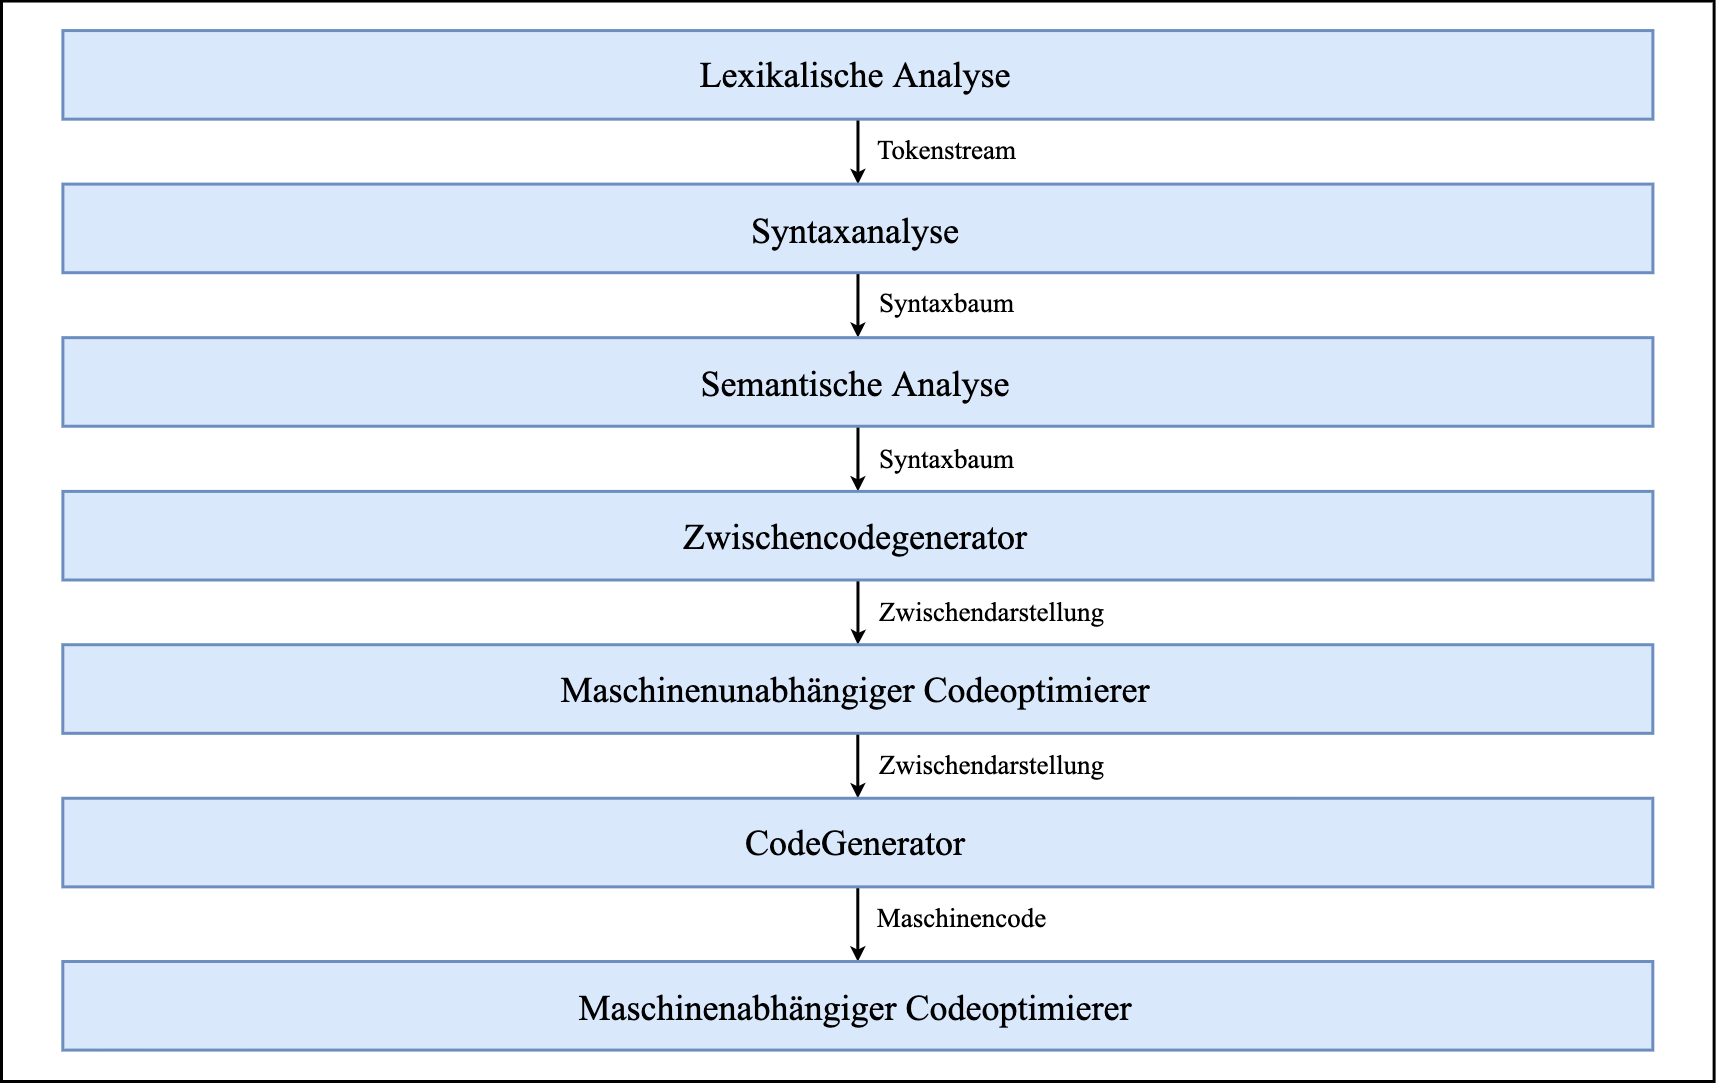
\includegraphics[width=14.5cm,height=9.15cm]{Images/Compiler/Phasen.png}
 \caption[Phasen eines Compilers]{Phasen eines Compilers\protect\footcite{Ullmann2008}}
 \label{fig:Compilerphasen}
\end{figure}
\footnotetext{Abbildung in Anlehnung an Ullman et al. 2008, S.6.}


\subsection{Lexikalische Analyse}
Die erste Phase eines Compilers ist die lexikalische Analyse die sich mit der Untergliederung des Quelltextes in Lexeme beschäftigt.  Ein Lexem ist die Folge von Zeichen im Quellprogramm,  die als Instanz eines Tokens erkannt wurden.  Dabei ist ein Token ein Paar aus Namen und einem optionalen Attributwert wobei der Name zum Beispiel ein bestimmtes Schlüsselwort oder eine Folge von Eingabezeichen seien kann und der Attributwert auf einen Eintrag in der Symboltabelle zeigt.  \footcite[Vgl.][S. 135 f.]{Ullmann2008} In Tabelle \ref{tab:Tokens} werden einige Beispielhafte Tokens aufgeführt und aus welchen Lexemen diese extrahiert werden.

\begin{table}[!ht]
\begin{tabularx}{\textwidth}{l|X|l}
   \textbf{Token} & \textbf{Beschreibung} & \textbf{Lexem} \\
\hline
if             & Zeichen i,f           & if                      \\ 
comparison     & Vergleichsoperatoren  & \textless{}=            \\ 
id             & Buchstaben            & pi                      \\ 
number         & Numerische Konstanten    & 3.14159                  
\end{tabularx}
\caption[Token-Beispiele]{Token-Beispiele \protect\footcite{Ullmann2008}}
 \label{tab:Tokens}
\end{table}
\footnotetext{Vgl. Ullman et al.  2008, S. 137.}

Basierend auf dieser Beschreibung ist in \ref{fig:LexerResult} ein Beispiel dargestellt, welches zeigt wie der Lexer aus einem Zeichenstring mehrere Token mit den optionalen Attributwerten generiert.  
 
\begin{figure}[!ht]
 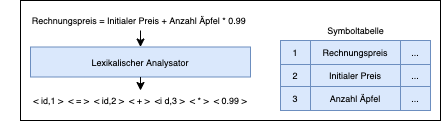
\includegraphics[width=14.5cm,height=3cm]{Images/Compiler/LexerResult.png}
 \caption[Lexer Beispiel]{Lexer Beispiel\protect\footcite{Ullmann2008}}
 \label{fig:LexerResult}
\end{figure}
\footnotetext{Abbildung in Anlehnung an Ullman et al. 2008, S.10.}

Der Lexer interagiert mit den anderen Komponenten eines Compilers, diese  Beziehungen werden in Abbildung \ref{fig:LexerInteraktionen}  dargestellt.  Dabei wird der Lexer häufig durch den Parser aufgerufen,  dies wird in der Abbildung mit dem Aufruf "getNextToken" dargestellt.  \footcite[Vgl.][S. 135]{Ullmann2008} 

\begin{figure}[!ht]
 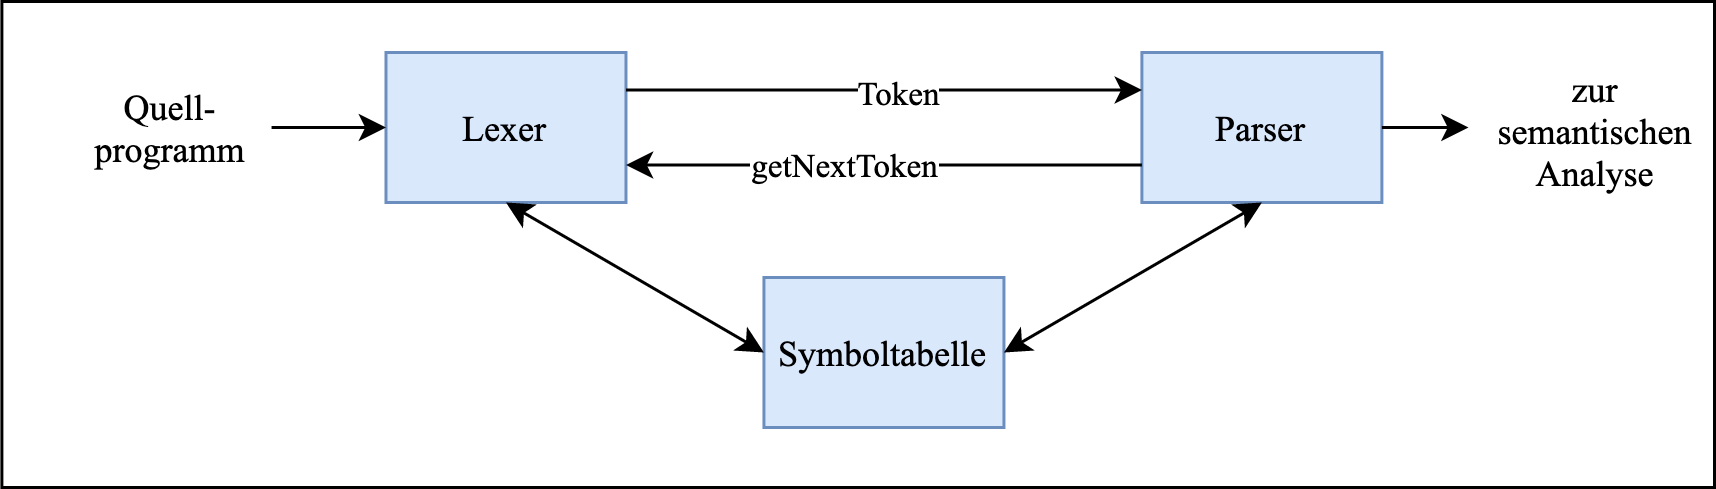
\includegraphics[width=14.5cm,height=4.11cm]{Images/Compiler/LexerParser.png}
 \caption[Interaktion zwischen Lexer und Parser]{Interaktion zwischen Lexer und Parser\protect\footcite{Ullmann2008}}
 \label{fig:LexerInteraktionen}
\end{figure}


Da der Lexer derjenige Teil des Compilers ist, der den Quelltext liest, kann er neben der Identifikation von Lexemen auch weitere Aufgaben übernehmen. So eignet er sich Ideal zum Streichen von Kommentaren im Quelltext und zum entfernen von Leerstellen wie Leerzeichen und Tabulatoren.  Eine weitere essentielle Aufgabe des Lexers ist es eine Zuordnung von Zeilennummern zu gefunden Fehlern herstellen zu können.  Bei einem Fehler wärend der Kompilierung kann somit ein Fehler an den Entwickler ausgegeben werden mit einem genauen Hinweis,  wo der Fehler aufgetreten ist. \footnotetext{Abbildung in Anlehnung an Ullman et al. 2008, S.135.} \footcite[Vgl.][S. 135.]{Ullmann2008} 
Häufig werden Lexer daher in zwei Kaskadierende Prozesse unterteilt, einem Löschen von Kommentaren und Zusammenfassen von Leerraumzeichen und einen für die eigentliche lexikalische Analyse.  \footcite[Vgl.][S. 136.]{Ullmann2008} 

\subsection{Syntaxanalyse}
Die zweite Phase des Compilers ist die Syntaxanalye in welcher der sogenannte Parser oder auch syntaktischer Analysator genannt die vom lexikalischen Analysator ausgegebenen Token in eine baumartige Zwischendarstellung überführt, die die grammatische Struktur der Tokens zeigt.  Diese Darstellung wird basierend auf ihrem Aussehen häufig als Syntaxbaum bezeichnet.  Die Knoten im Syntaxbaum stehen für eine Operation und die Kindknoten für die Argumente dieser Operation.  Die Anordnung der Operationen stimmt mit üblichen arithmentischen Konventionen überein,  wie zum Beispiel der Vorrang der Multiplikation vor Addition. \footcite[Vgl.][S. 9]{Ullmann2008} Abbildung \ref{fig:ParserResult} zeigt die Erstellung eines Syntaxbaumes Anhand von einer Reihe von Token, dabei wurden die Tokens aus dem Beispiel der Abbildung  \ref{fig:LexerResult} übernommen.  Anhand des Knotens <id, 1> ist jederzeit über die Symboltabelle bekannt,  dass das Ergebnis der Rechnung an den Speicherort des Bezeichners Rechnungspreis abgelegt werden muss. \footcite[Vgl.][S. 9.]{Ullmann2008} 

\begin{figure}[!ht]
 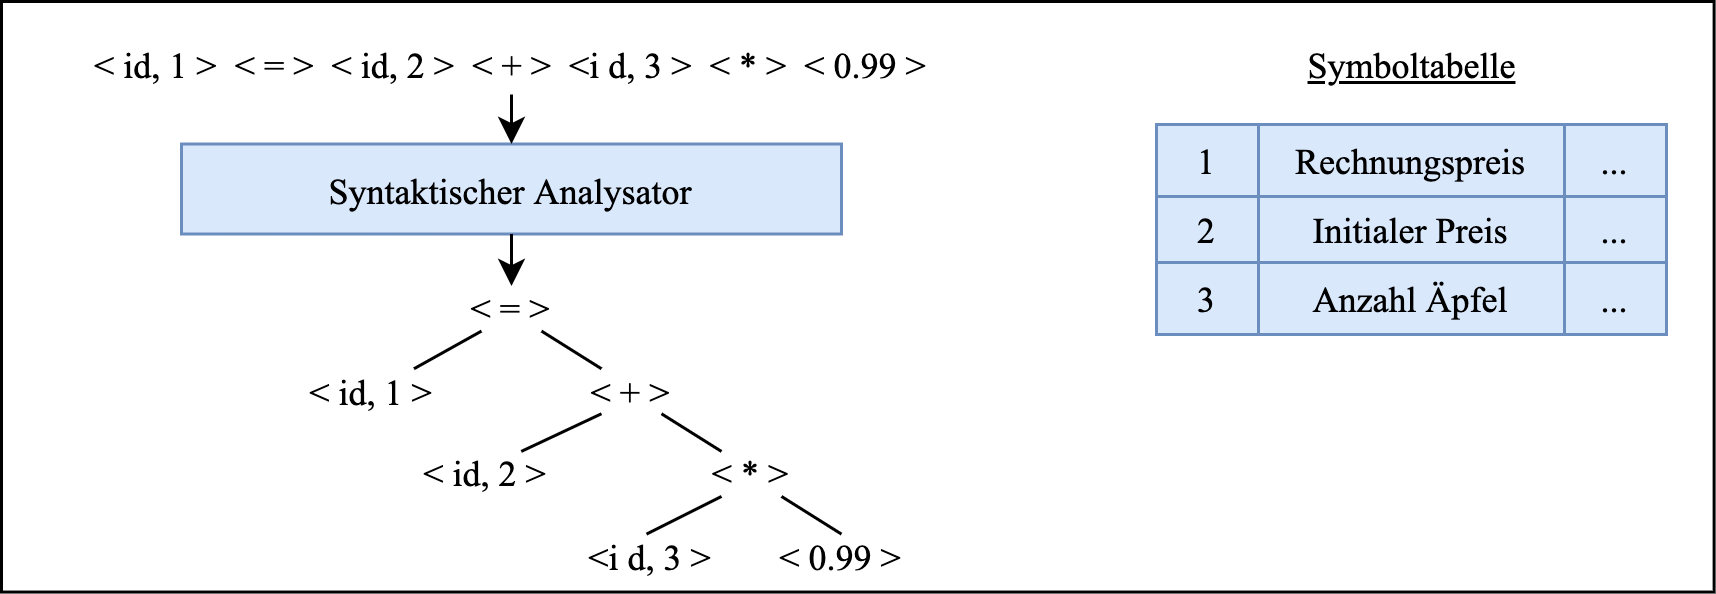
\includegraphics[width=14.5cm,height=5cm]{Images/Compiler/ParserResult.png}
 \caption[Syntaxbaum]{Syntaxbaum \protect\footcite{Ullmann2008} }
 \label{fig:ParserResult}
\end{figure}
\subsection{Semantische Analyse}

Bei der semantischen Analyse wird der Syntaxbaum,  \footnotetext{Abbildung in Anlehnung an Ullman et al. 2008, S.10.}  als Aufgliederung der Programmkonstruktur,  zusammen mit den Informationen aus der Symboltabelle verwendet um das Quellprogramm auf semantische Konsistenz mit der Sprachdefinition zu überprüfen. \footcite[Vgl.][S. 157]{Wilhelm2012}.  Außerdem werden in dieser Typinformationen gesammelt und entweder im Syntaxbaum oder in der Symboltabelle hinterlegt um sie in späteren Phasen zu verwenden. Dabei werden außerdem Typen überprüft,  daher analysiert ob jeder Operator die passenden Operanden hat.  So wird beispielsweise geprüft wird, ob ein Arrayindex ein Integer ist. Auch Typkonvertierungen können können zu dieser Zeit innerhalb des Baumss hinterlegt werden.  So wurde in dem bisherigen Beispiel die Anzahl Äpfel als Ganzzahl behandelt und wird für die Berechnung des Preises in Abbildung \ref{fig:Typ} zu Float konvertiert. \footcite[Vgl.][S. 9ff]{Ullmann2008}

\begin{figure}[!ht]
 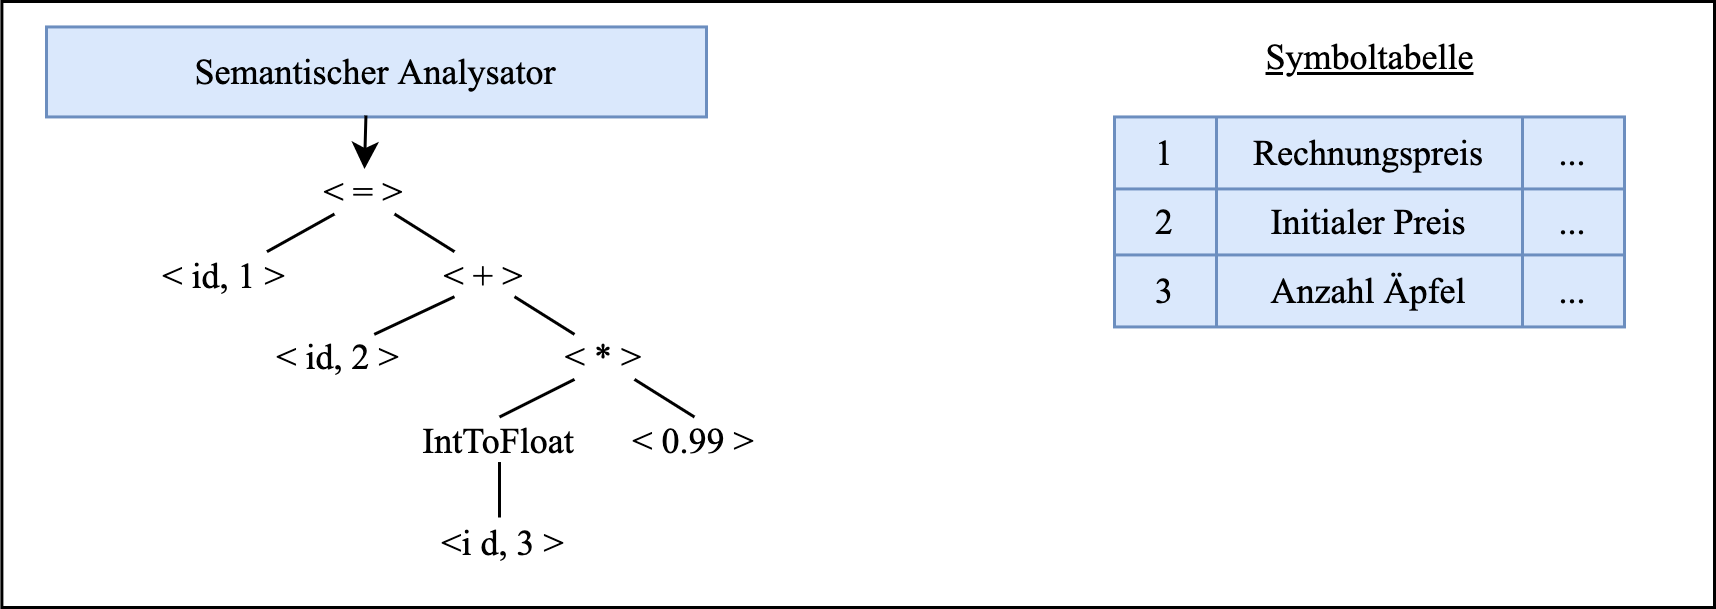
\includegraphics[width=14.5cm,height=5cm]{Images/Compiler/Type.png}
 \caption[Typüberprüfung]{Typüberprüfung \protect\footcite{Ullmann2008} }
 \label{fig:Typ}
\end{figure}
\footnotetext{Abbildung in Anlehnung an Ullman et al. 2008, S.10.} 
\subsection{Zwischencodeerzeugung}
Bei der Übersetzung eines Quellprogramms in den Zielcode kann der Compiler mehrere Zwischendarstellungen in verschiedenen Formen erstellen. Syntaxbäume sind beispielsweise eine solche Darstellung. Nach der semantischen Analyse stellen viele Compiler eine maschinennahe Zwischendarstellung die für eine Abstrakte Maschine entworfen wurden.  Darstellungen niedriger Ebene sind für maschinenabhängige Aufgaben, z. B. Registerabgabe und Befehlsauswahl, geeignet.
\begin{figure}[!ht]
 
\includegraphics[width=14.5cm,height=1.52cm]{Images/Compiler/Zwischendarstellungen.png}
 \caption[Zwischendarstellungen]{Zwischendarstellungen \protect\footcite{Ullmann2008} }
 \label{fig:Zwischendarstellung}
\end{figure}
\footnotetext{Abbildung in Anlehnung an Ullman et al. 2008, S.433.} 

Die Auswahl oder der Entwurf einer Zwischendarstellung ist von Compiler zu Compiler  unterschiedlich.  Eine Zwischendarstellung kann entweder eine tatsächliche Sprache  sein oder aus internen Datenstrukturen bestehen, die von den Phasen des Compilers gemeinsam verwendet werden. Auch wenn C eine Programmiersprache ist, wird sie häufig  als eine Zwischenform verwendet, da sie flexibel ist, zu effizienten Maschinencode kompiliert werden kann und ihre Compiler weitgehend verfügbar sind.\footcite[Vgl.][S. 433]{Ullmann2008}


\subsection{Codeoptimierung}
In dieser Phase wird der Code so optimiert, dass sich darauf ein besserer Zielcode ergibt.  Dabei bedeutet besser, schnellerer code oder code der weniger Ressourcen verbraucht.  Der Umfang der Codeoptimierung schwankt dabei von Compiler zu Compiler erheblich.  \footcite[Vgl.][S. 11f]{Ullmann2008} Wenn ein Programmierer erst einmal einen bestimmten Algorithmus ausgewählt  und implementiert hat, kann der Compiler außer in ganz besonderen Fällen nicht genug  vom Programm verstehen, um ihn durch einen anderen, effizienteren Algorithmus zu  ersetzen.\footcite[Vgl.][S. 712]{Ullmann2008}

\subsection{Codeerzeugung}
Bei der Codeerzeugung werden die Eingaben aus der Zwischendarstellung des Quellprogramms entgegengenommen und auf die Zielsprache abgebildet. Das Zielprogramm  muss die semantische Bedeutung des Quellprogramms bewahren und qualitativ hochwertig sein, also die verfügbaren Ressourcen der Zielmaschine effizient nutzen.  Die Herausforderung ist, dass das Problem, für ein gegebenes Quellprogramm ein optimales Zielprogramm zu erstellen, mathematisch nicht entscheidbar ist; zahlreiche  Teilprobleme, die bei der Codeerzeugung anfallen, zum Beispiel die Vergabe von Registern, sind nicht effizient berechenbar (intractable). In der Praxis müssen wir mit heuristischen Techniken zufrieden sein, die guten, aber nicht unbedingt optimalen Code liefern.  Im Allgemeinen können die  Codeoptimierungs- und die Codeerzeugungsphase, die zusammen häufig als Back-End  des Compilers bezeichnet werden, die IR mehrmals durchlaufen, bevor das Zielprogramm steht. \footcite[Vgl.][S. 618f]{Ullmann2008}

\section{Der .NET Compiler Roslyn}
Für die Arbeit mit der Programmiersprache C\# steht mit Roslyn ein Compiler zur Verfügung, der aus modularen Bibliotheken zusammensetzen. Durch die Referenzierung dieser Bibliotheken können Programme in verschiedenen Art und Weisen auf die Funktionalitäten des Compilers zugreifen.  So ist es auch Möglich, den Compiler zu verwenden ohne das Ziel zu haben die Programmiersprache C\# zu plattformnahen Code zu übersetzen.  Dabei steht die Bibliotheken über den Packetemanager Nuget für die Einbindung in eigene Projekte zur Verfügung.  Um diese Funktionalität zu gewährleisten unterteilt Rosyln die Übersetzung in mehrere Phasen die einige der in diesem Kapitel beschriebenen Phasen zusammenfassen: Die erste Phase ist die Erstellung des Syntaxbaums, die zweite Phase ist die Semantische Analyse gefolgt von der letzten Phase der Ausgabe der so genannten Intermediate Language. \footcite[Vgl.][S. 1017]{Albahari2020}



